\documentclass{article}
\usepackage{graphicx}
\usepackage{amsmath}
\usepackage{subcaption}
\usepackage{amsfonts}
\usepackage[makeroom]{cancel}
\usepackage{hyperref}

\title{TEK5600 - Obligatory Assignment}
\author{Edvart G. Bjerke}
\date{March 2025}

\begin{document}

\maketitle

\section{Field Lines}
A field line is both a mathematical object and a tool commonly used to visualize
vector fields. Field lines are curves that are tangent to the underlying vector field
at all points. The vector field defines a system of first-order differential equations, and the field lines are particular solutions to this system.

In this report, the vector field in question is a time-independent \\
2-dimensional vector field representing velocity.
Given an initial position, the field line is a parametric curve that represents the streamline of the flow, showing the path of an imaginary particle.

In practice, the solutions are not found analytically, but are simulated using 
numerical integration schemes on a discretized version of the vector field.
In this case, the domain of the vector function is discretized into an $N \times M$ grid of points.
The values at the exact grid points are samples of the true vector fields. To be able to
sample in between grid points, an interpolation scheme is used. For this project, bilinear interpolation has been implemented. 

\begin{figure}[h!]
    \centering
    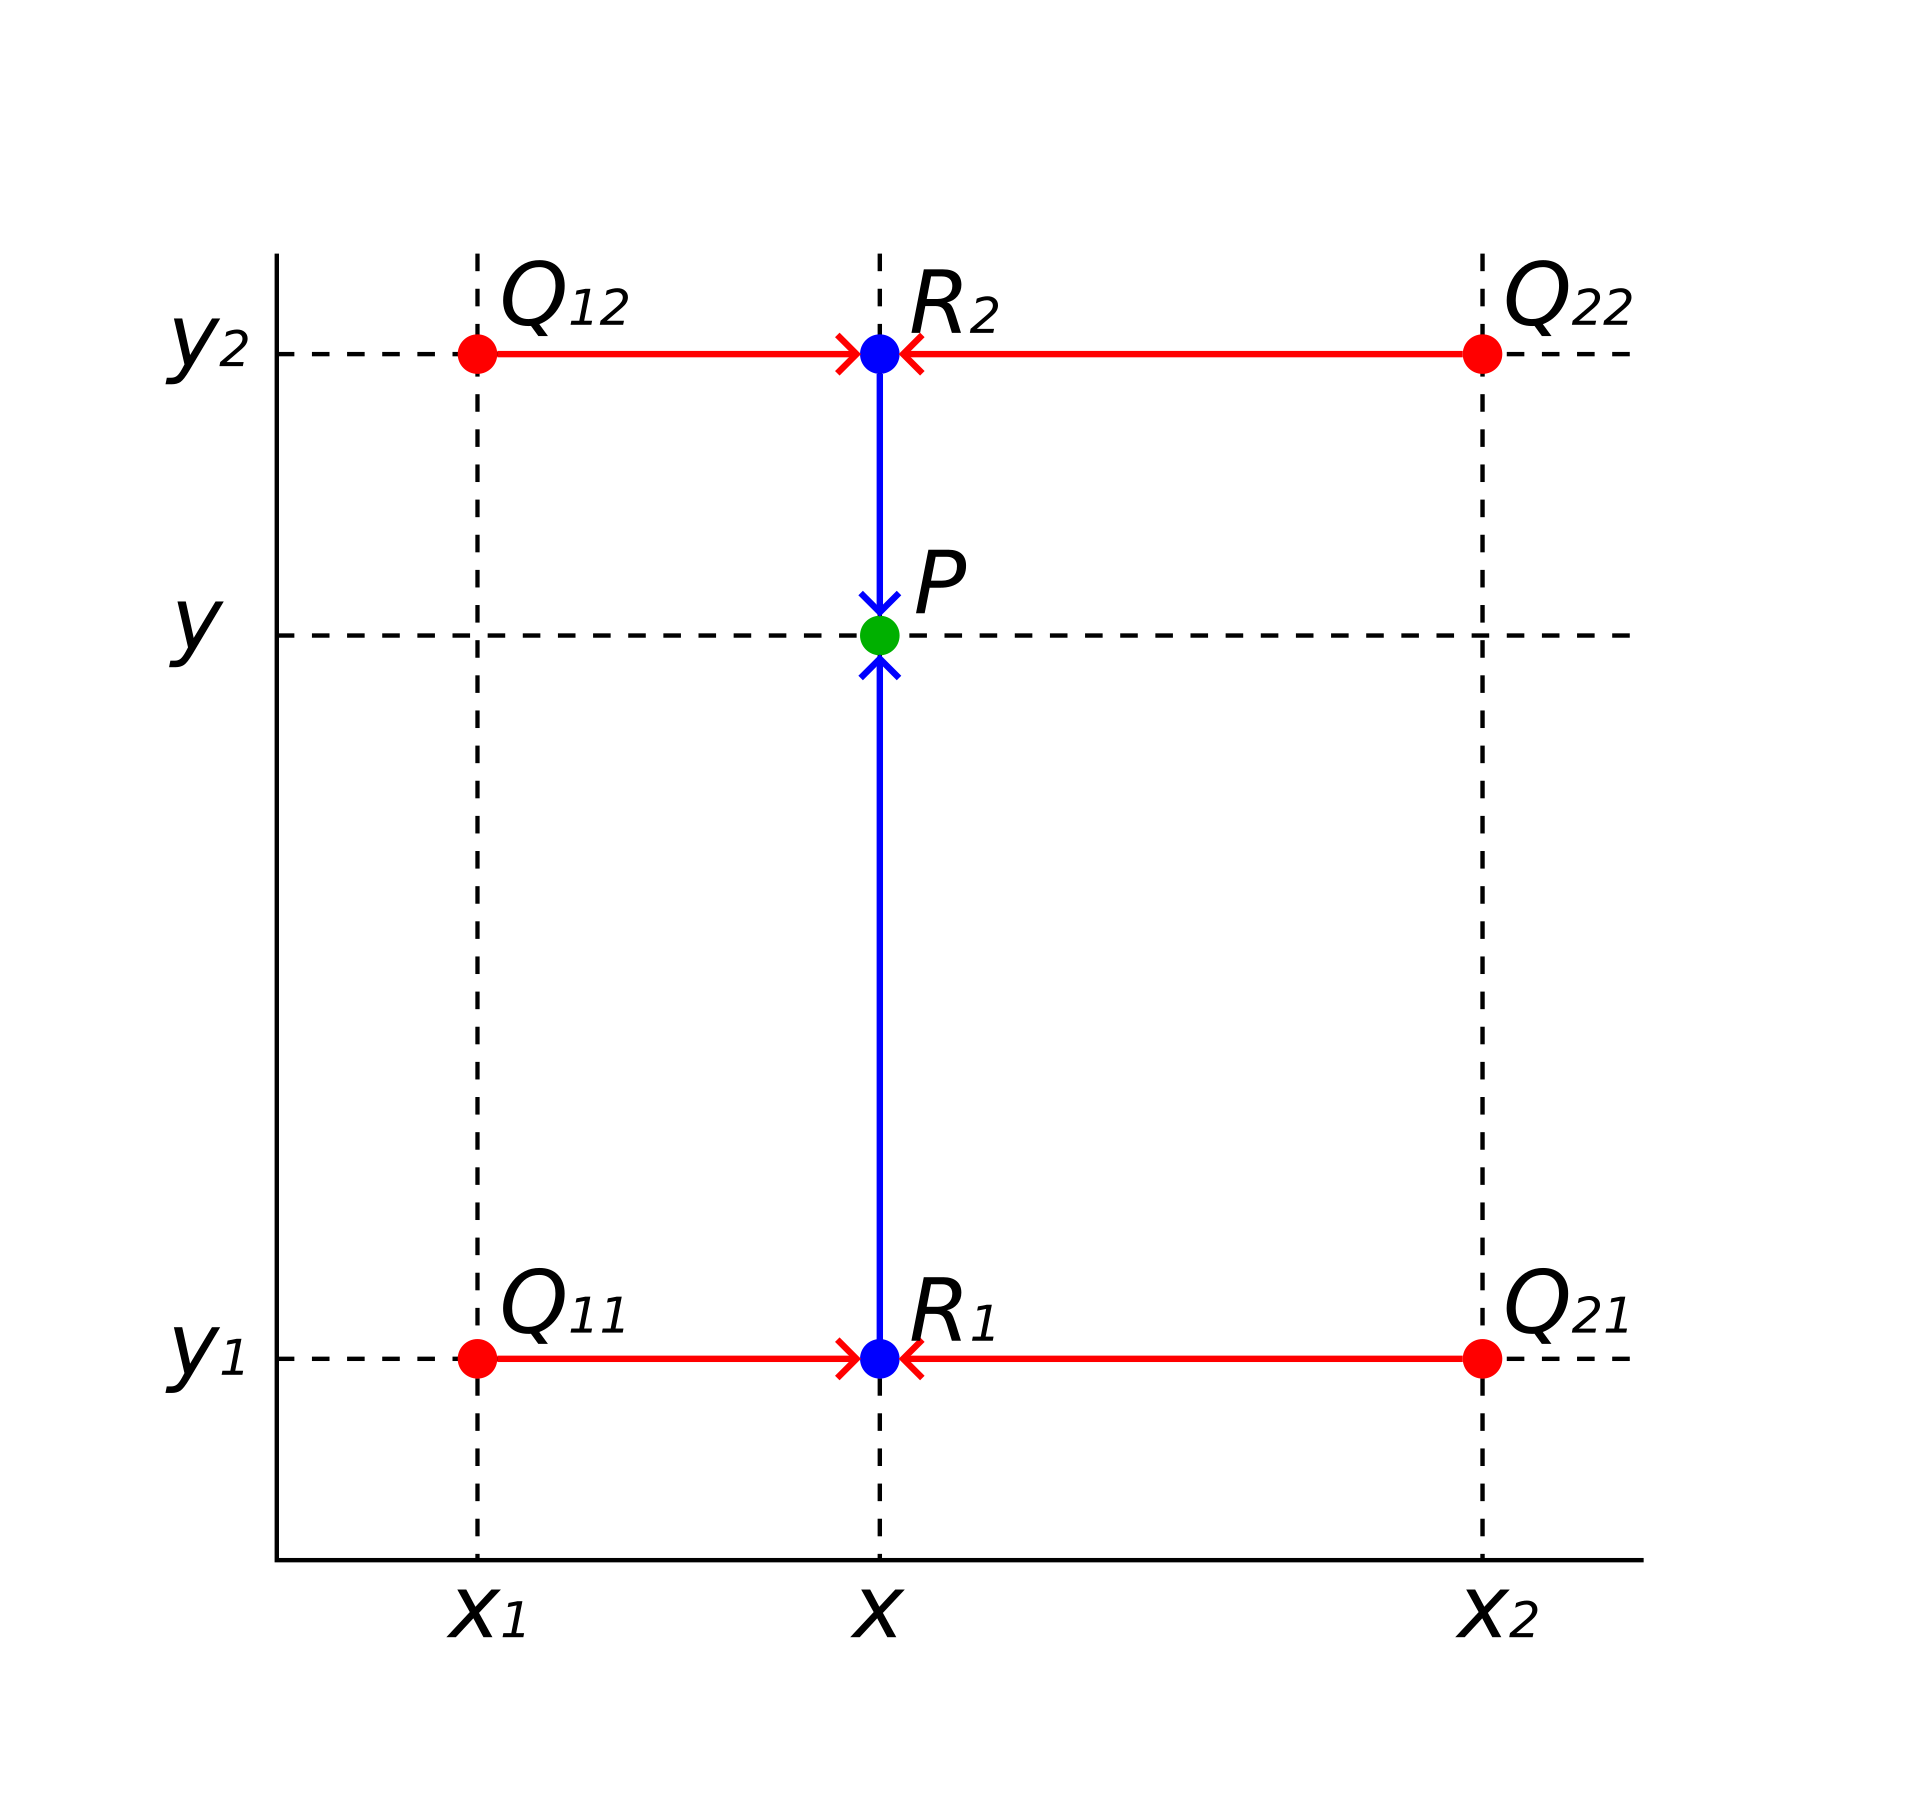
\includegraphics[width=0.5\textwidth]{BilinearInterpolationV2.svg.png}
    \caption{Bilinear interpolation. The sampled point $P$ is a weighted sum of the four nearest grid points.}
\end{figure}

\subsection{Integration schemes}
Two integration schemes were used to find particular solutions: the forward euler method and the Runge-Kutta (RK4) method.

The (time-independent) vector field $V$ is defined as a function which takes in a position vector  $(x, y)$, and returns a velocity vector $(u, v)$ representing the velocity at that position:
$$V : \mathbb{R}^2 \rightarrow \mathbb{R}^2 $$
$$\mathbf{V}(\mathbf{x}(t)) = \begin{bmatrix}
    u(\mathbf{x}(t)) \\
    v(\mathbf{x}(t))
\end{bmatrix}, \quad
\mathbf{x} = \begin{bmatrix}
    x\\y
\end{bmatrix}
$$

The velocity field $V$ represents the ordinary differential equation relating 
the position vector $\mathbf{x}$ and its derivative:
$$\mathbf{x}'(t) = V(\mathbf{x}(t))$$
With solution:
$$\mathbf{x}(t) = \mathbf{x}(t_0) + \int_{t_0}^{t} \mathbf{V}(\mathbf{x(\tau)}) d\tau$$
Equations on this formed can be solved numerically using the forward euler method and RK4.

The euler method is derived by taking the first-order taylor approximation around $t = t_0$:
\begin{align*}
    \mathbf{x}(t) &\approx \mathbf{x}(t_0) + \mathbf{V}(\mathbf{x}(t_0))(t-t_0)\\
    &= \mathbf{x}(t_0) + h\mathbf{V}(\mathbf{x}(t_0)) 
\end{align*}
Where $h = (t-t_0)$ is the step size. The error of the solution decreases as the step length is reduced.
The equation is solved iteratively by integrating one "step ahead" at a time:
$$\mathbf{x}_{k+1} = \mathbf{x}_k + hV(\mathbf{x}_k)$$

RK4 is similar to the euler method, but evaluates the derivative four times for each integration step:
$$\mathbf{x}_{k+1} = \mathbf{x}_k + \frac{h}{6}(k_1+k_2+k_3+k_4)$$
$$k_1 = \mathbf{V}(\mathbf{x}_k)$$
$$k_2 = \mathbf{V}\left(\mathbf{x}_k+\frac{h}{2}k_1\right)$$
$$k_3 = \mathbf{V}\left(\mathbf{x}_k+\frac{h}{2}k_2\right)$$
$$k_4 = \mathbf{V}\left(\mathbf{x}_k+hk_3\right)$$

\subsection{Seeding strategies}
The seeding strategy is the scheme used to select initial positions for the numerical DE solver. 
A good seeding strategy is one that is fast and captures the most important features without causing clutter.
For this assignment, three seeding strategies have been implemented.

\subsubsection{Random seeding}
Random seeding is a simple strategy where seed points are generated randomly based on some distribution.
Here, a uniform distribution was used to generate positions spanning the size of the grid.
\begin{verbatim}
for i in range(num_particles):
    seeds_x.append(np.random.random() * u.shape[0] - 2)
    seeds_y.append(np.random.random() * u.shape[0] - 2)
\end{verbatim}

\newpage

\begin{figure}[h!]
    \centering
    \begin{subfigure}{0.65\textwidth}
        \centering
        
\includegraphics[width=\textwidth]{metsim_random_150.eps}
        \caption{150 randomly seeded streamlines}
    \end{subfigure}
    \hfill
    \hfill
    \begin{subfigure}{0.65\textwidth}
        \centering
        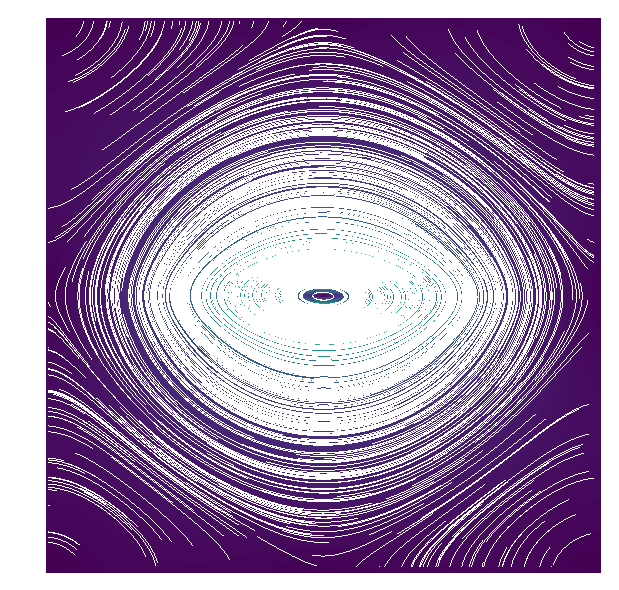
\includegraphics[width=\textwidth]{metsim_random_500.eps}
        \caption{500 randomly seeded streamlines}
    \end{subfigure}
    \caption{Random seeding on metsim data (vector graphics, zoom in!)}
\end{figure}


\begin{figure}[h!]
    \centering
    \begin{subfigure}{0.65\textwidth}
        \centering
        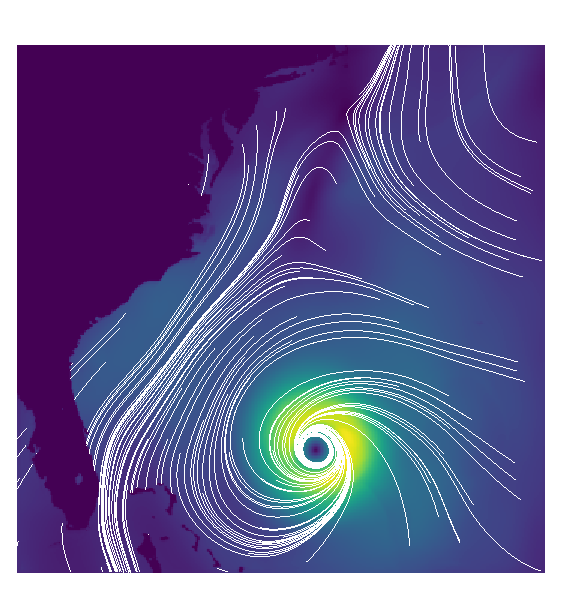
\includegraphics[width=\textwidth]{isabel_random_150.eps}
        \caption{150 randomly seeded points}
    \end{subfigure}
    \hfill
    \hfill
    \begin{subfigure}{0.65\textwidth}
        \centering
        
\includegraphics[width=\textwidth]{isabel_random_500.eps}
        \caption{500 randomly seeded points}
    \end{subfigure}
    \caption{Random seeding on isabel data (vector graphics, zoom in!)}
\end{figure}

\subsubsection{Uniform seeding}
Uniform seeding is another simple seeding strategy where seeds
are uniformly distributed (evenly spaced) onto the domain.

\begin{figure}[h!]
    \centering
    \begin{subfigure}{0.6\textwidth}
        \centering
        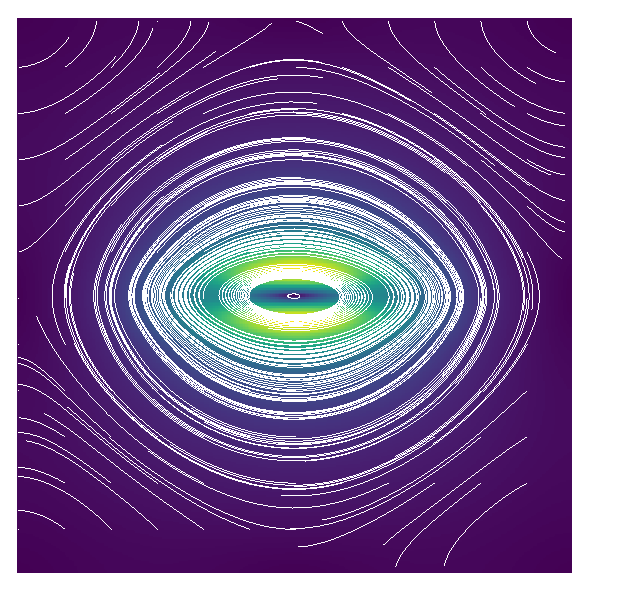
\includegraphics[width=\textwidth]{metsim_uniform_150.eps}
        \caption{150 uniformly seeded streamlines}
    \end{subfigure}
    \hfill
    \hfill
    \begin{subfigure}{0.6\textwidth}
        \centering
        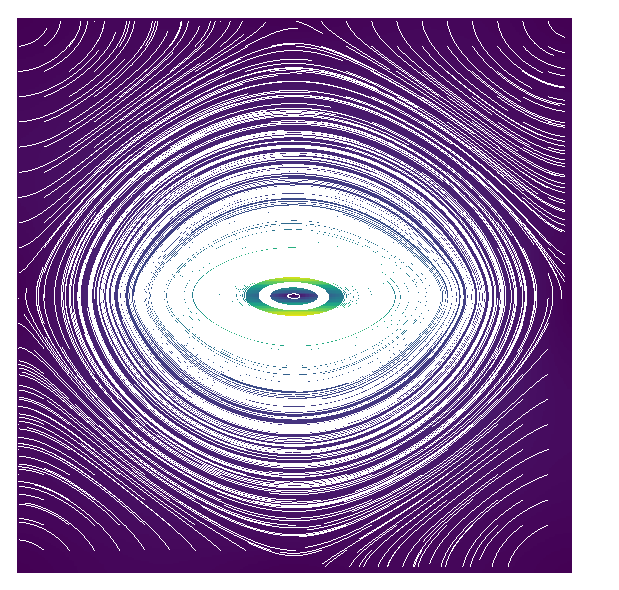
\includegraphics[width=\textwidth]{metsim_uniform_500.eps}
        \caption{500 uniformly seeded streamlines}
    \end{subfigure}
    \caption{Uniform seeding on metsim data}
\end{figure}

\newpage
\begin{figure}[h!]
    \centering
    \begin{subfigure}{0.6\textwidth}
        \centering
        
\includegraphics[width=\textwidth]{isabel_uniform_150.eps}
        \caption{150 uniformly seeded streamlines}
    \end{subfigure}
    \hfill
    \hfill
    \begin{subfigure}{0.6\textwidth}
        \centering
        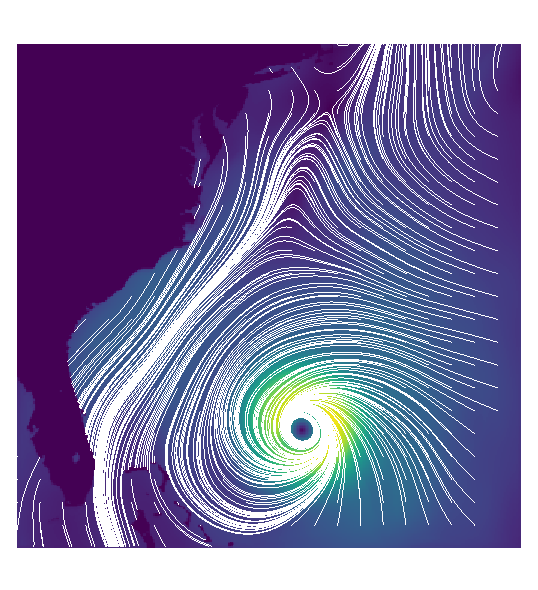
\includegraphics[width=\textwidth]{isabel_uniform_500.eps}
        \caption{500 uniformly seeded streamlines}
    \end{subfigure}
    \caption{Uniform seeding on isabel data}
\end{figure}


\subsubsection{Vorticity-based seeding}
In this custom seeding strategy, the vorticity of the vector field is used
to generate seeding points. The vorticity $\mathbf{\omega}$ is defined as the curl of the velocity field:
\begin{align*}
    \mathbf{\omega} &= \nabla \times \mathbf{v} \\
    &= \nabla \times \left[u(x, y), v(x, y)\right] \\
    &= \frac{\partial v}{\partial x} - \frac{\partial u}{ \partial y}
\end{align*}
The vorticity of a 2-dimensional velocity field is a vector field pointing purely in the z-direction. In this implementation, 
the magnitude of this vector field is used to generate a probability map from which seed points are randomly sampled.
Gaussian blurring has been applied to the vorticity map and a bias has been added such that even areas with close to zero vorticity are 
represented in the field line visualization.

One can also experiment with modifying the vorticity map using the power operator. Powers greater than 1 will increase the contrast
(highlight the center of the tornado) while powers less than one will equalize the vorticity map.

To compute the vorticity map, the \verb|np.gradient()| was used, which computes the derivatives of the velocity field
using second order central differences.


\begin{figure}[h!]
    \centering
    \begin{subfigure}{0.32\textwidth}
        \centering
        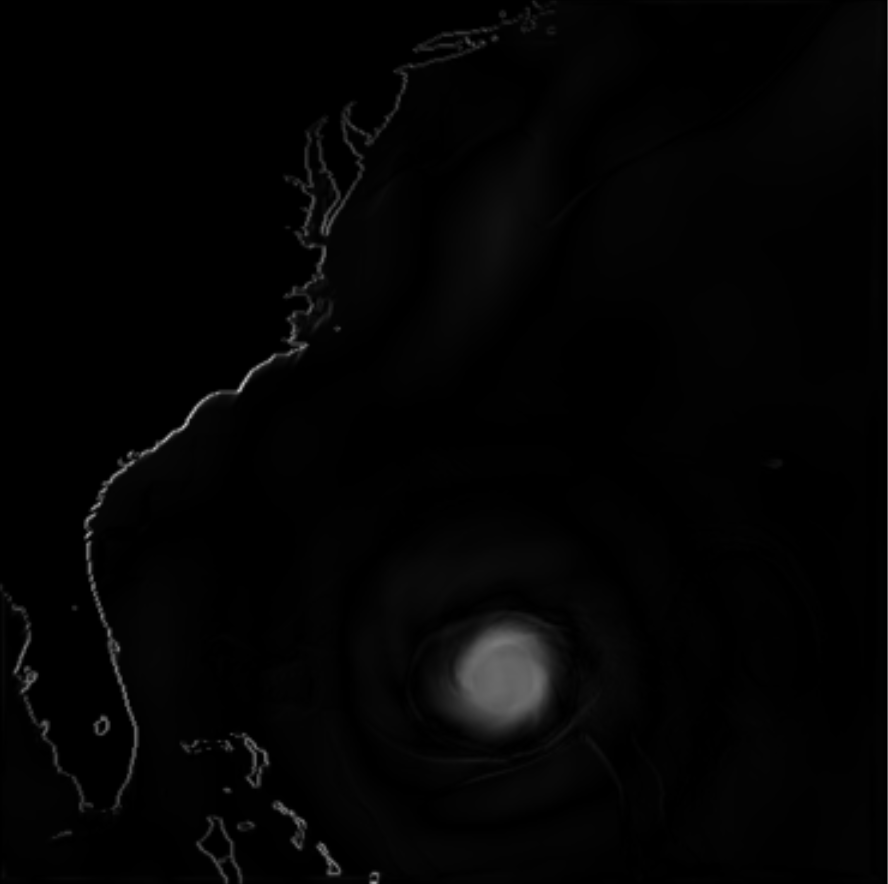
\includegraphics[width=\textwidth]{vorticity_map.png}
        \caption{Vorticity magnitude field.}
    \end{subfigure}
    \hfill
    \begin{subfigure}{0.32\textwidth}
        \centering
        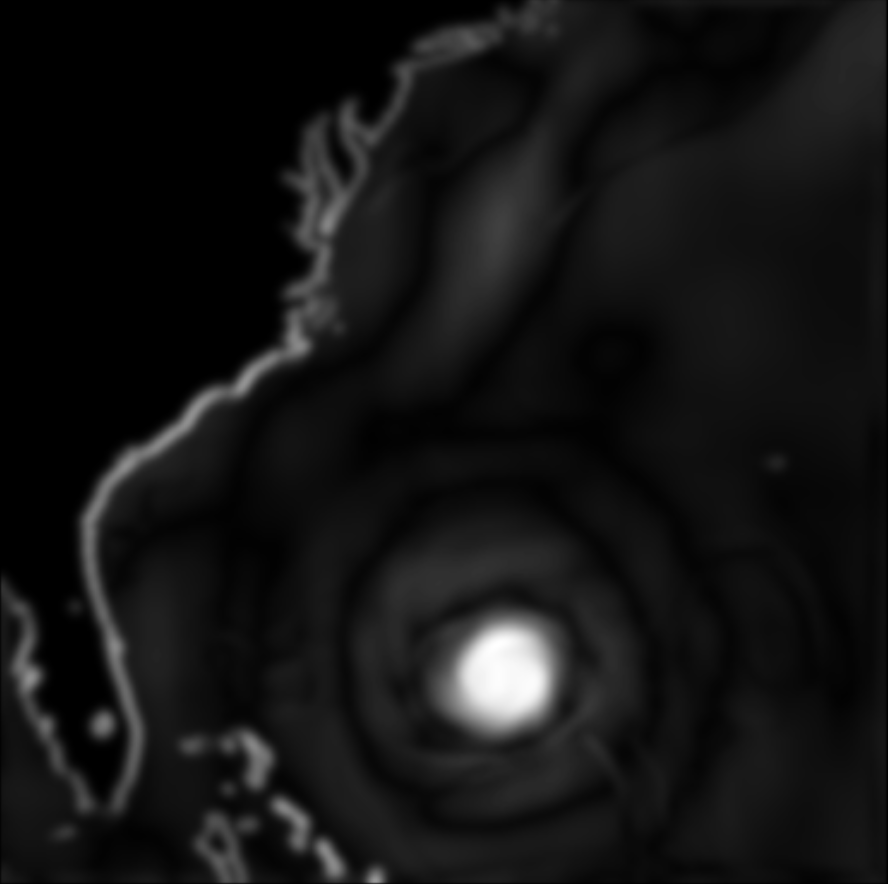
\includegraphics[width=\textwidth]{pow_0_6.png}
        \caption{Vorticity magnitude raised to 0.6.}
    \end{subfigure}
    \hfill
    \begin{subfigure}{0.32\textwidth}
        \centering
        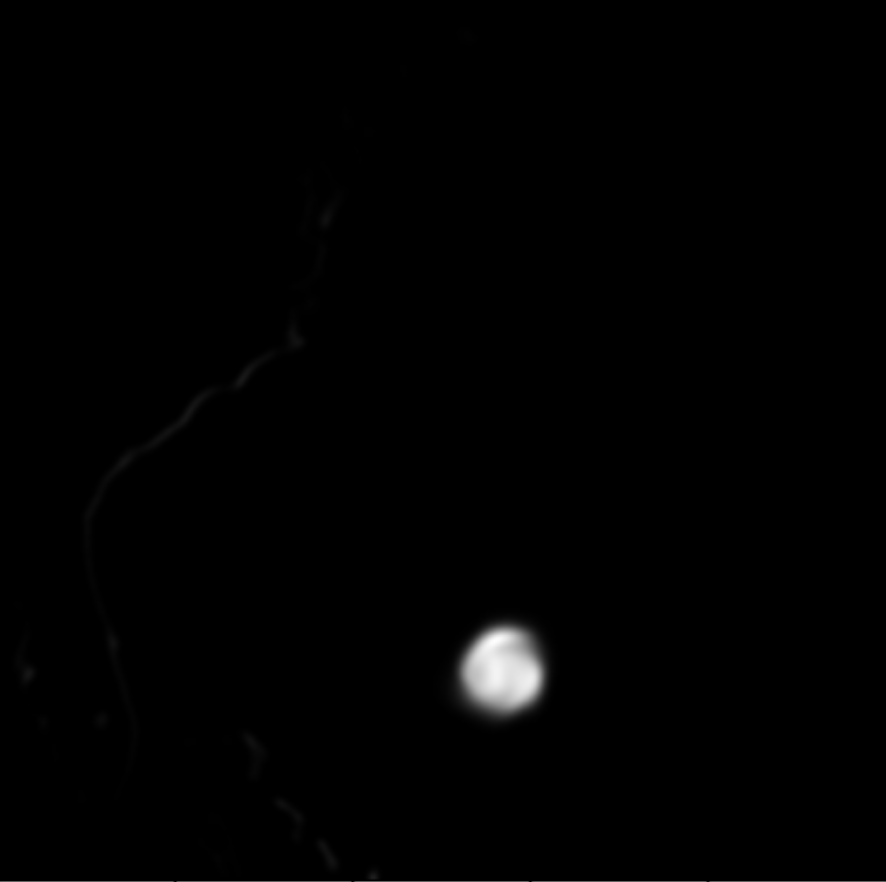
\includegraphics[width=\textwidth]{pow_3_0.png}
        \caption{Vorticity magnitude raised to 3.0.}
    \end{subfigure}
    \caption{Comparison of vorticity magnitude field transformations.}
\end{figure}

\newpage

\begin{figure}[h!]
    \centering
    \begin{subfigure}{0.65\textwidth}
        \centering
        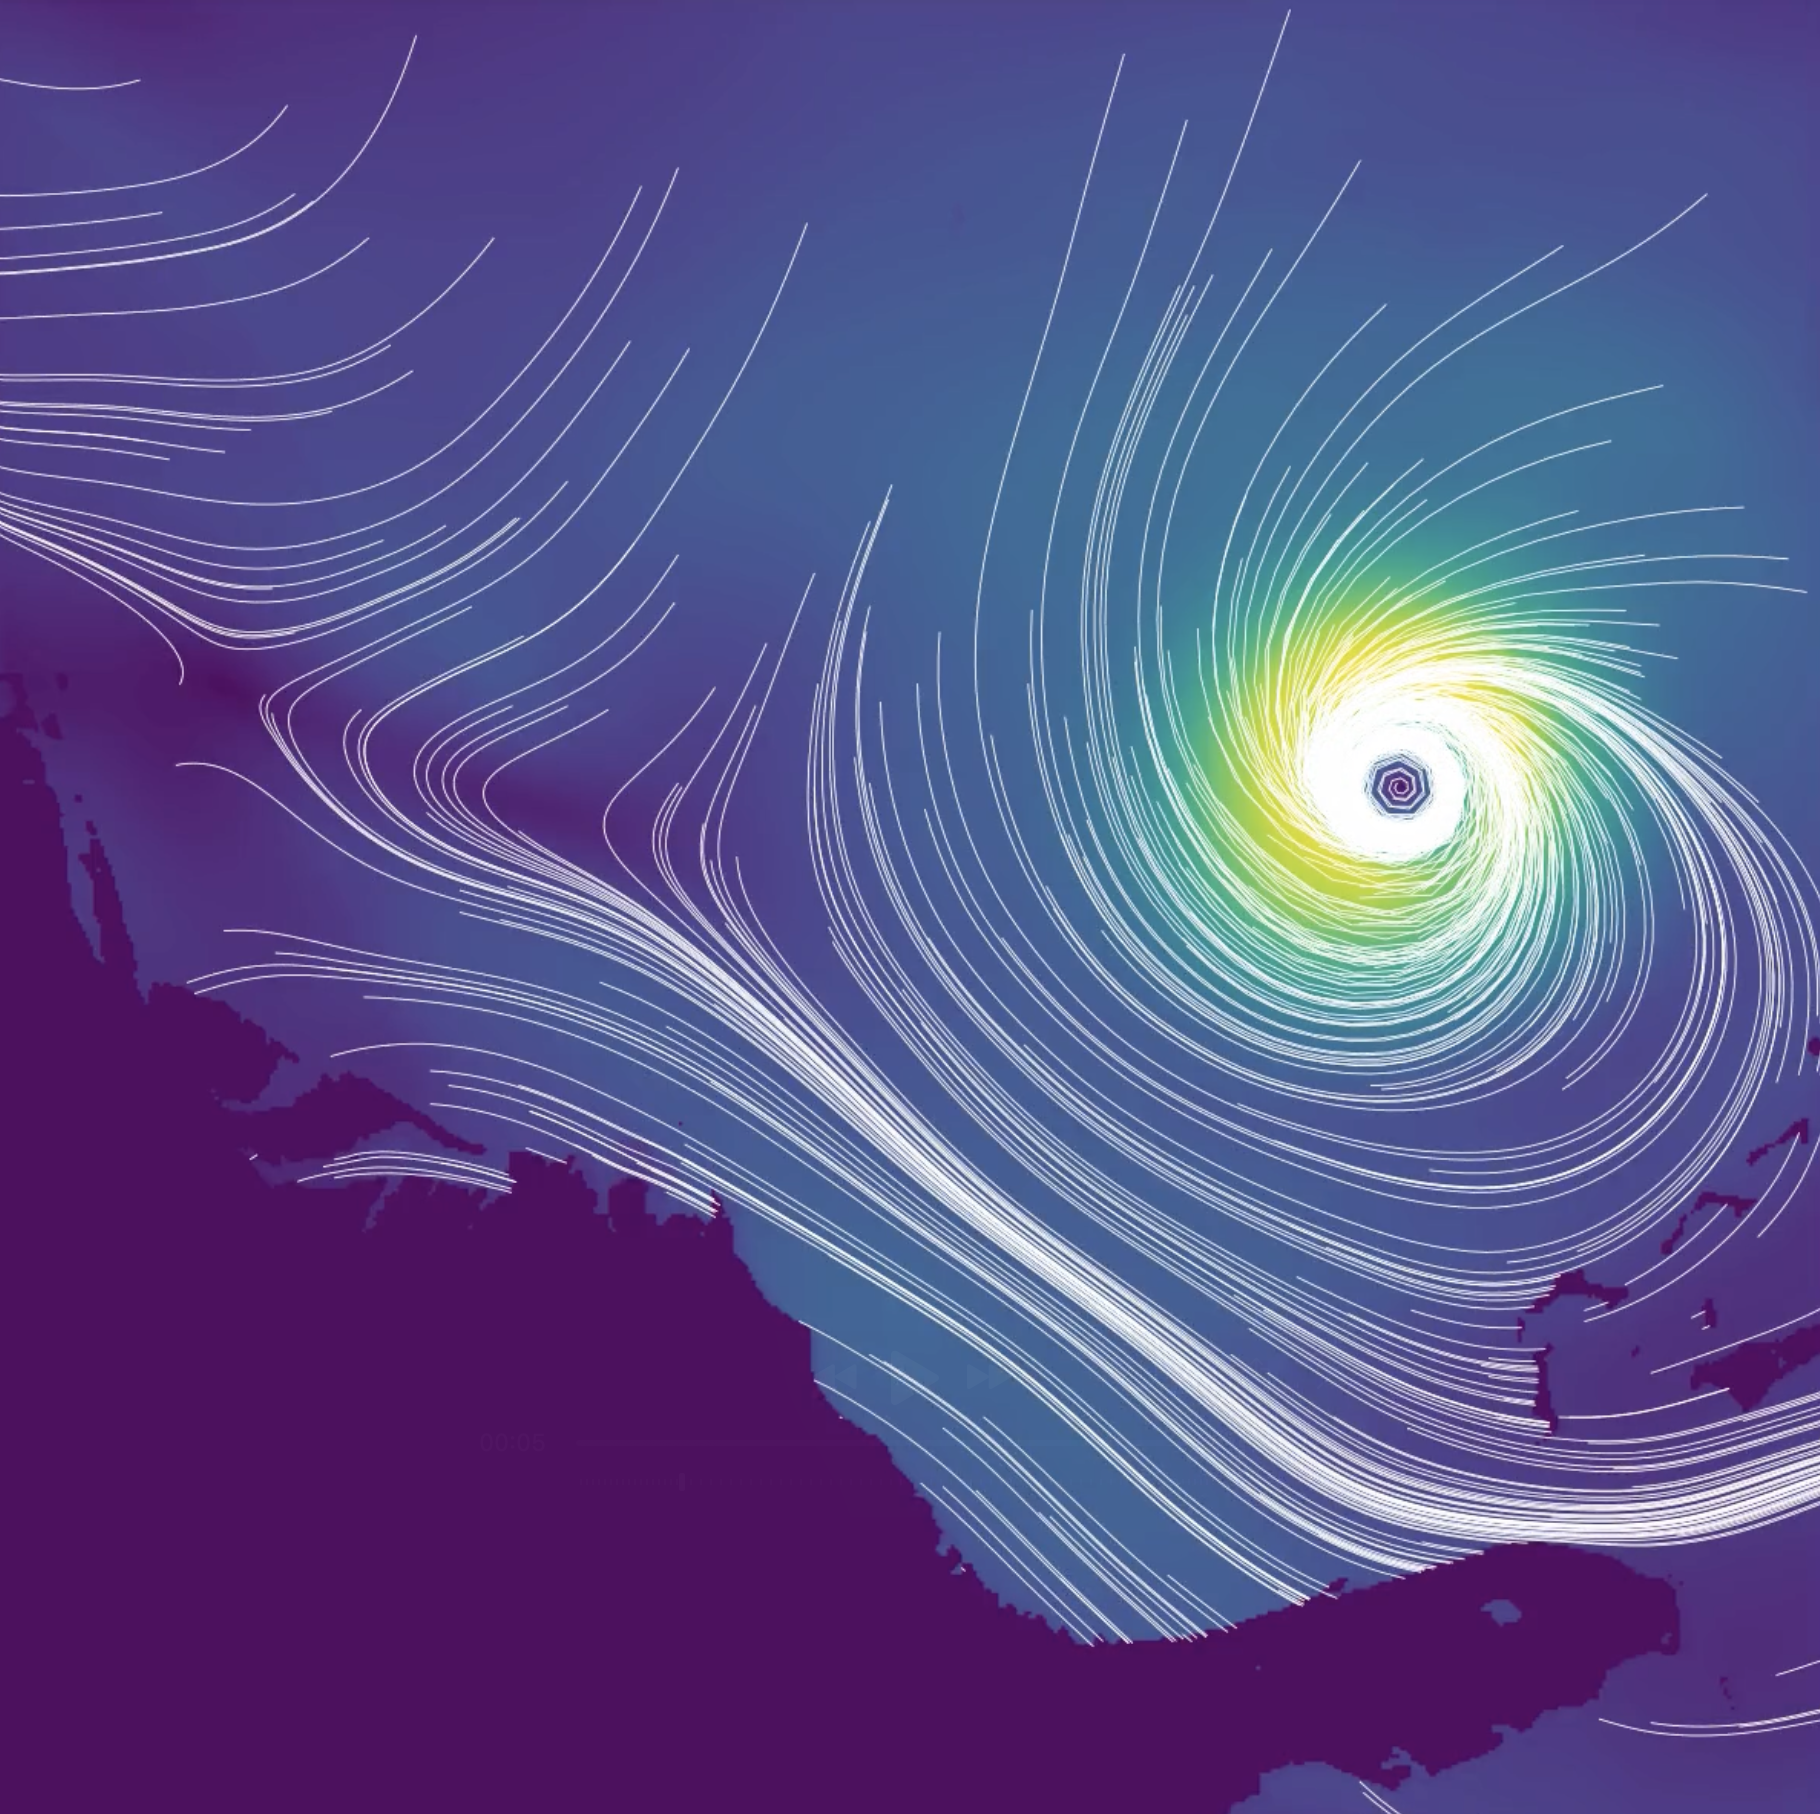
\includegraphics[width=\textwidth, angle=270]{vort_result.png}
        \caption{Field lines from vorticity map with flat bias}
    \end{subfigure}
    \hfill
    \begin{subfigure}{0.65\textwidth}
        \centering
        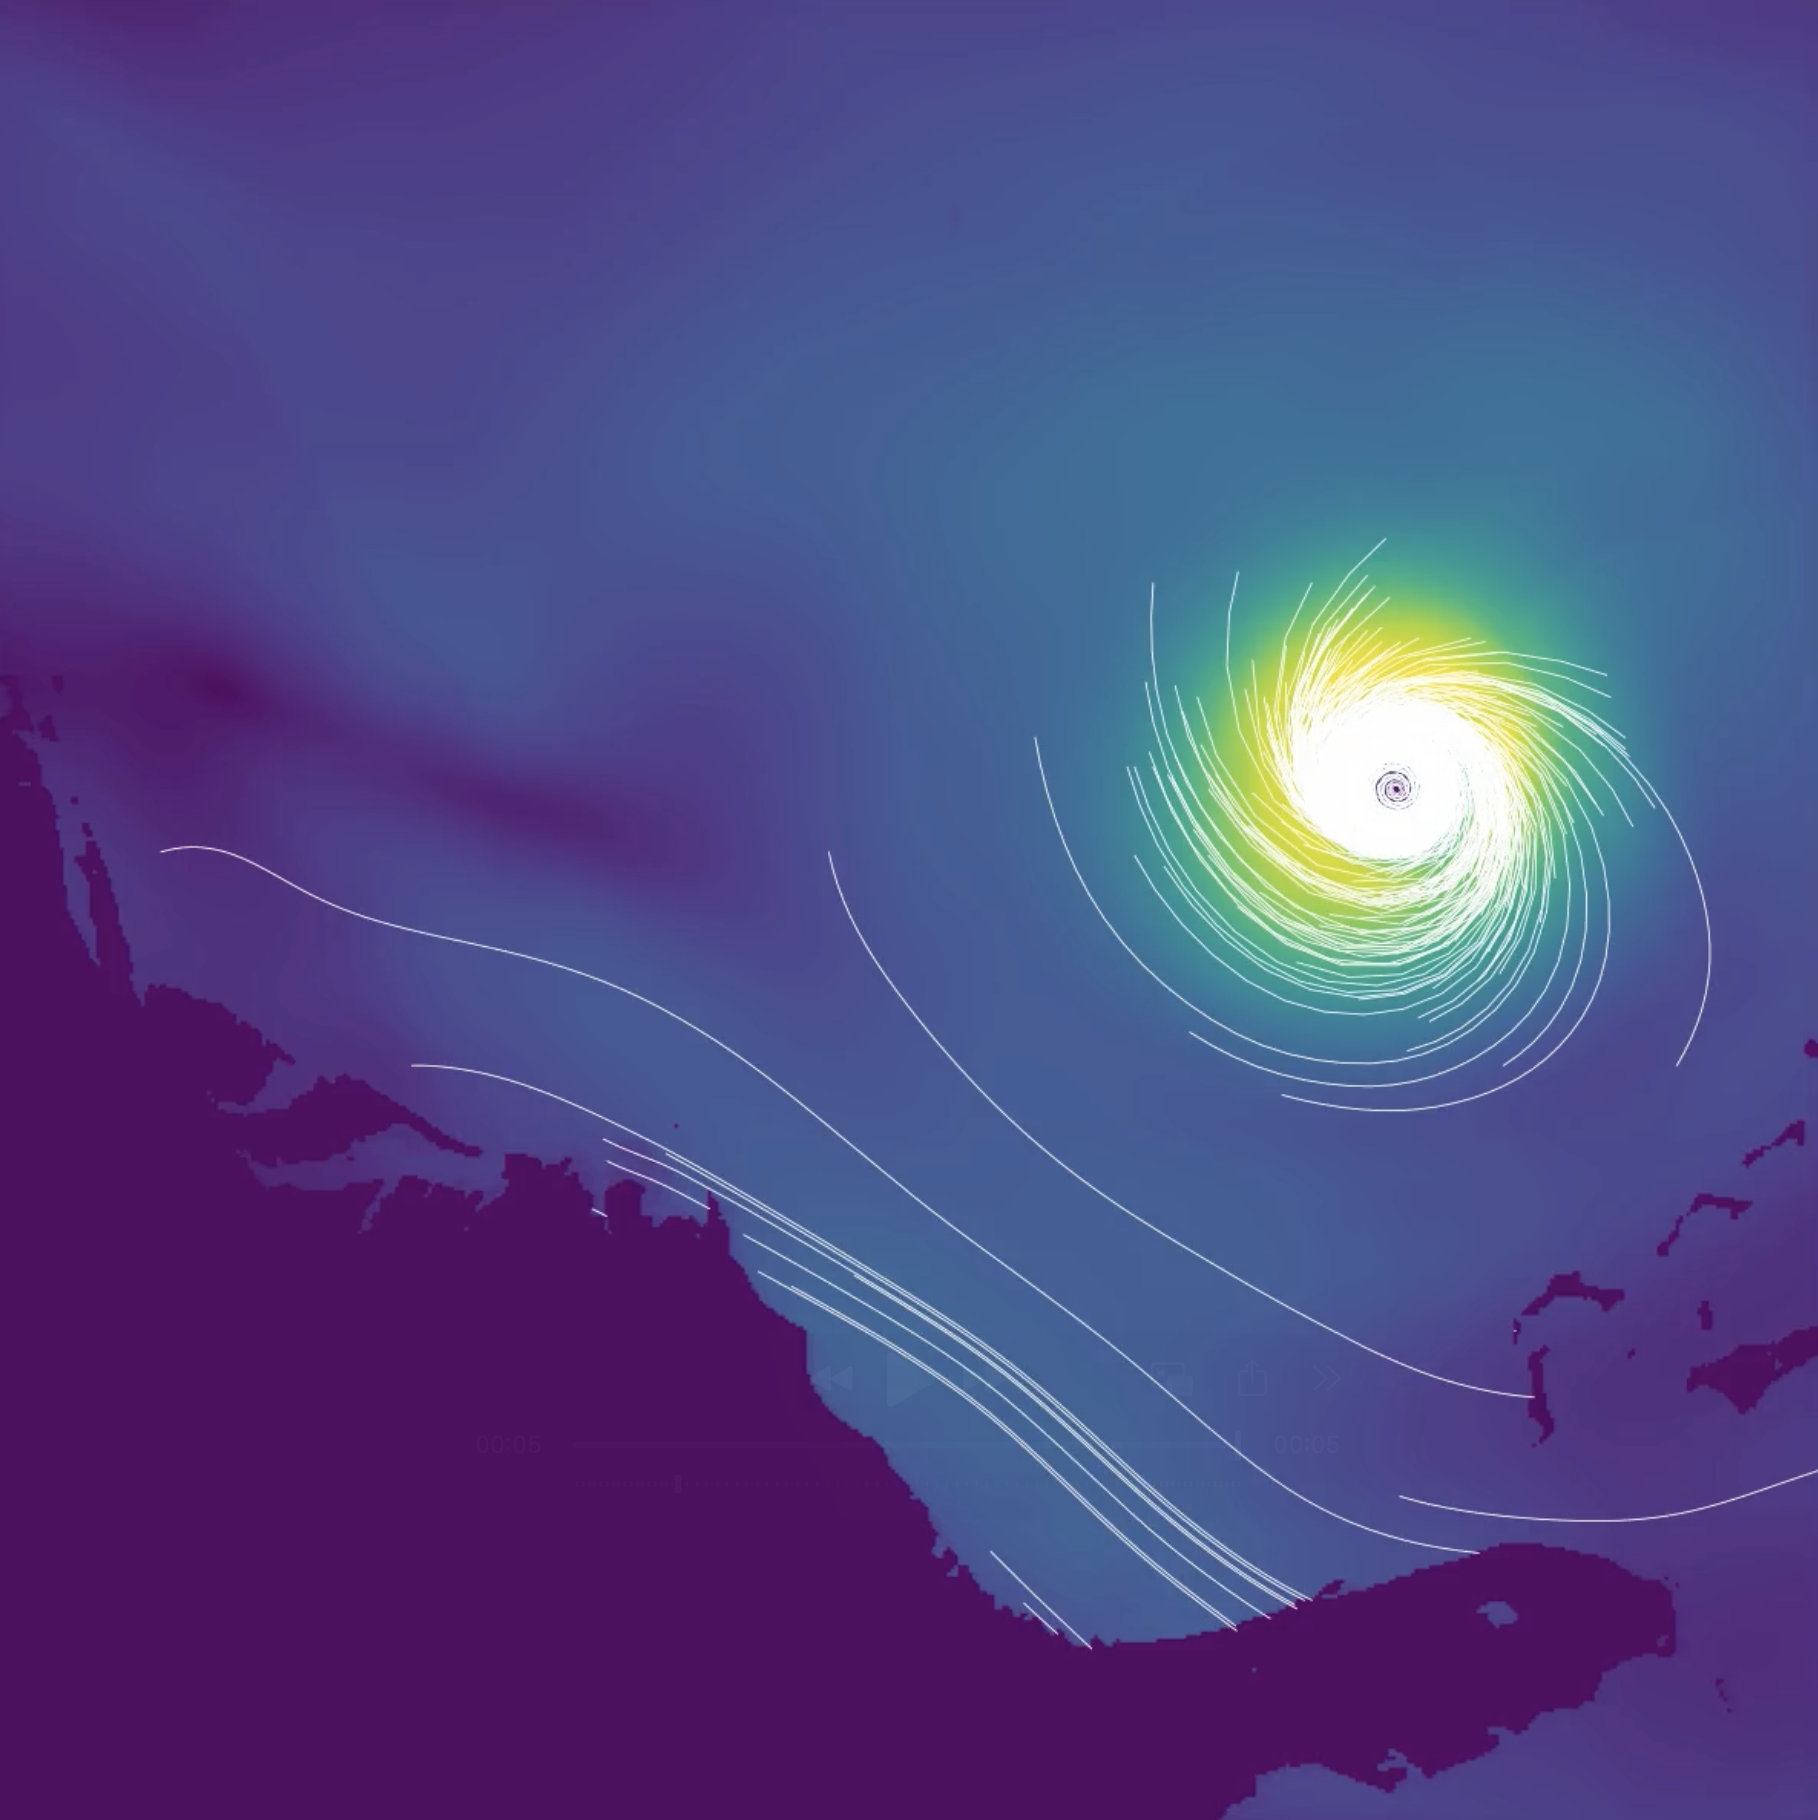
\includegraphics[width=\textwidth, angle=270]{vort_result_3_0.png}
        \caption{Field lines from vorticity map raised to 3.0}
    \end{subfigure}
    \caption{Vorticity-based seeding on isabel data}
\end{figure}

\newpage

\begin{figure}[h!]
    \centering
    \begin{subfigure}{0.48\textwidth}
        \centering
        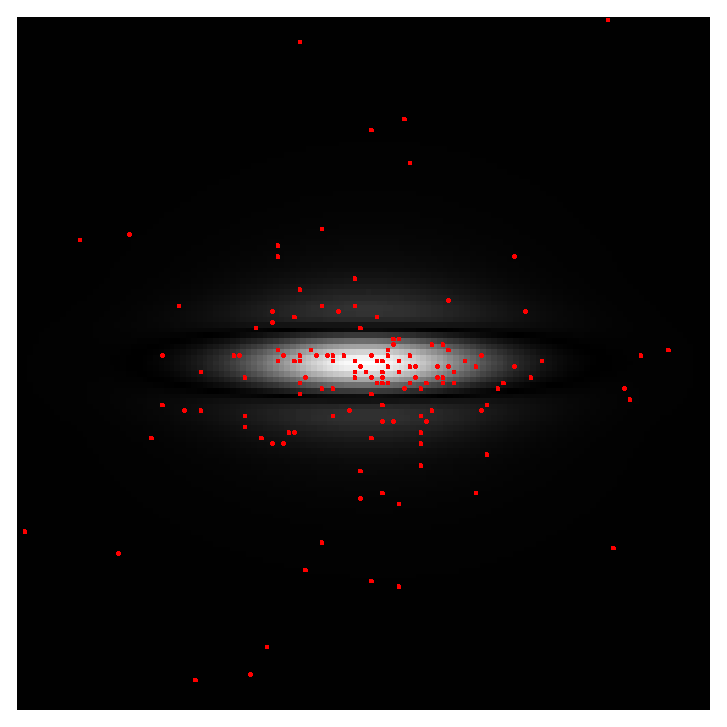
\includegraphics[width=\textwidth]{metsim_vorticity_unfiltered_seeds.eps}
        \caption{Unfiltered vorticity map with seed points}
    \end{subfigure}
    \hfill
    \begin{subfigure}{0.48\textwidth}
        \centering
        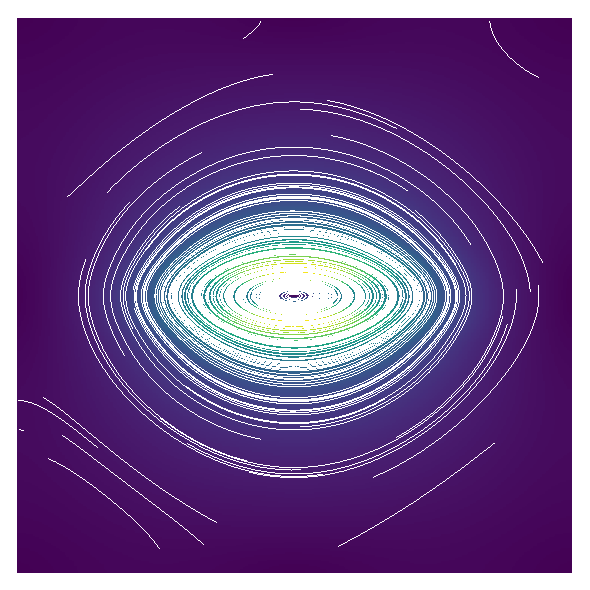
\includegraphics[width=\textwidth]{metsim_vorticity_unfiltered.eps}
        \caption{Resulting streamlines\vspace{3mm}}
    \end{subfigure}
    \caption{Unfiltered vorticity-based seeding on metsim data}
\end{figure}

\begin{figure}[h!]
    \centering
    \begin{subfigure}{0.43\textwidth}
        \centering
        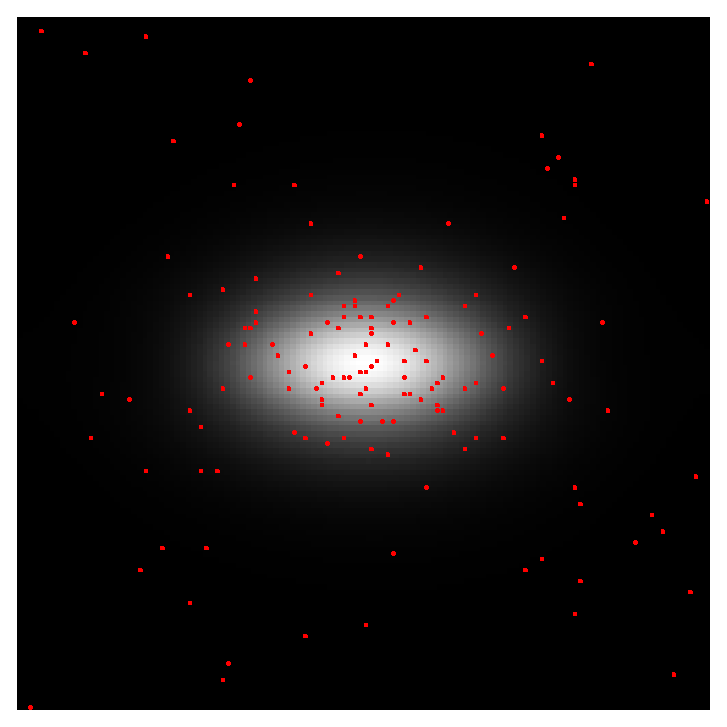
\includegraphics[width=\textwidth]{metsim_vorticity_filtered_seeds.eps}
        \caption{With blurring and added bias} % Add vertical space
    \end{subfigure}
    \hfill
    \begin{subfigure}{0.43\textwidth}
        \centering
        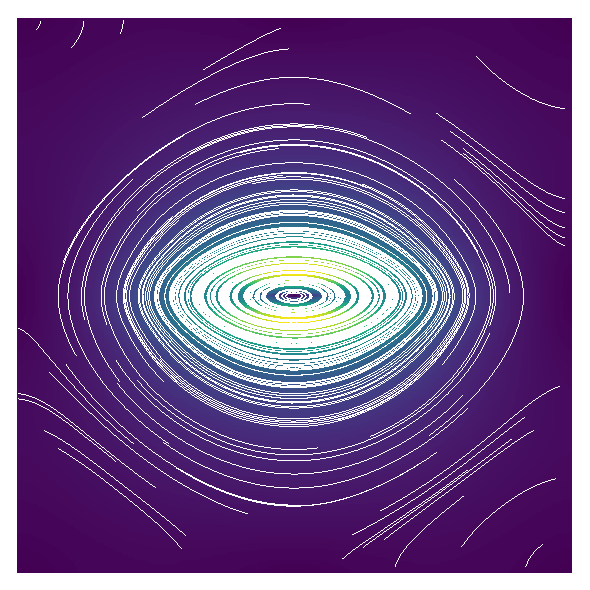
\includegraphics[width=\textwidth]{metsim_vorticity_filtered.eps}
        \caption{Resulting streamlines}
    \end{subfigure}
    \caption{Filtered vorticity-based seeding on metsim data. Vorticity was blurred with a gaussian kernel with $\sigma = 6$. A bias of $0.01*\mathrm{max}(\mathrm{vorticity})$ was also added.}
\end{figure}

All three strategies are able to highlight the general structures of the vector field, and it is difficult to say which one
is the most appropriate or useful. Overall, the uniform and random sampling strategies are very easy to implement, but give little control,
and no domain insight is used to highlight particular features. The vorticity-based sampling uses some domain insight (areas with high vorticity are more "interesting"), but
requires more computation and some tweaking to yield good results. Still, this allows for more control in how the sampling is done, and we might
get away with using fewer particles overall, reducing clutter.

The different integration schemes (Euler and RK4) were tested on the two vector fields. A coarse time step was used to highlight the difference in accuracy. The inaccuracy of Euler's method is particularly noticeable in regions with high vorticity, such as around the eye of the Isabel hurricane
\begin{figure}[h!]
    \centering
    \begin{subfigure}{0.48\textwidth}
        \centering
        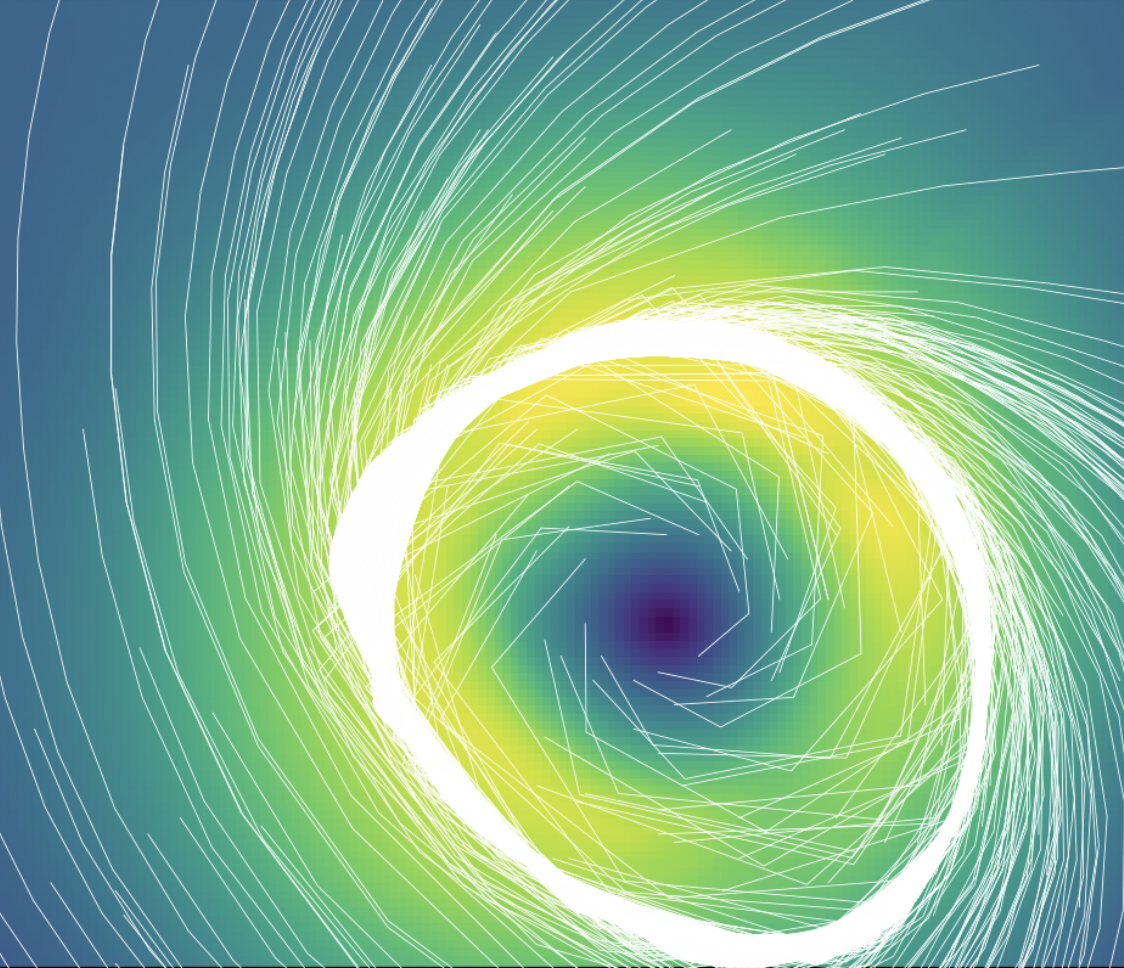
\includegraphics[width=\textwidth, angle=0]{euler.png}
        \caption{Euler}
    \end{subfigure}
    \hfill
    \begin{subfigure}{0.48\textwidth}
        \centering
        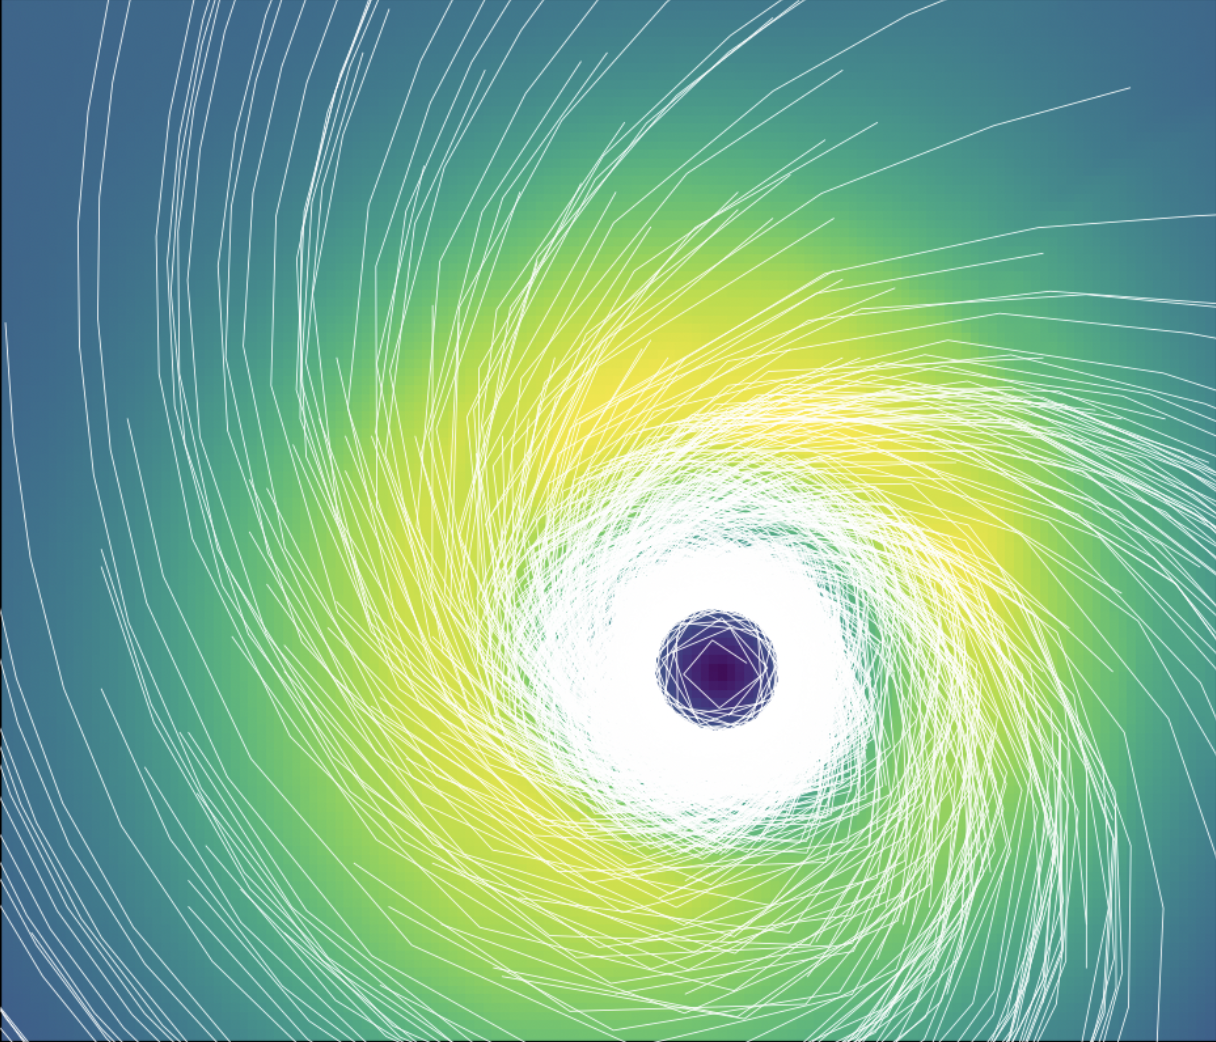
\includegraphics[width=\textwidth, angle=0]{rk4.png}
        \caption{RK4}
    \end{subfigure}
    \caption{Comparison of integration schemes on isabel data.}
\end{figure}

In the metsim data, the euler integration method results in overshooting, leading to a spiralling pattern. In these results,
the nature of the vector field could be misinterpreted.

\begin{figure}[h!]
    \centering
    \begin{subfigure}{0.48\textwidth}
        \centering
        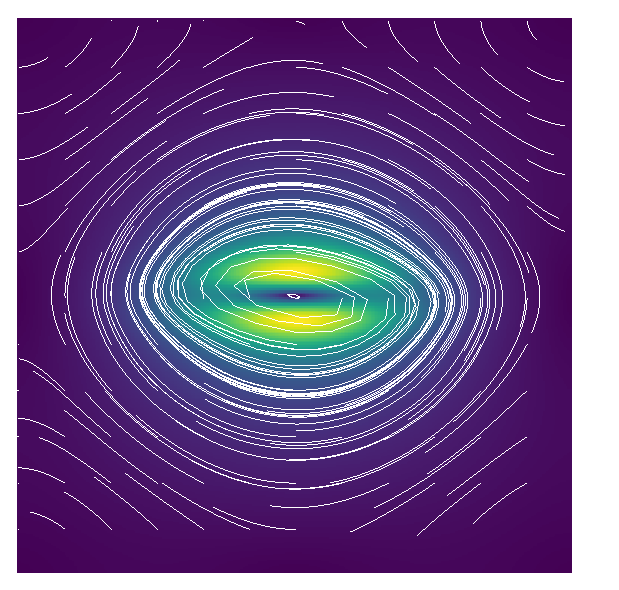
\includegraphics[width=\textwidth, angle=0]{metsim_uniform_euler.eps}
        \caption{Euler}
    \end{subfigure}
    \hfill
    \begin{subfigure}{0.48\textwidth}
        \centering
        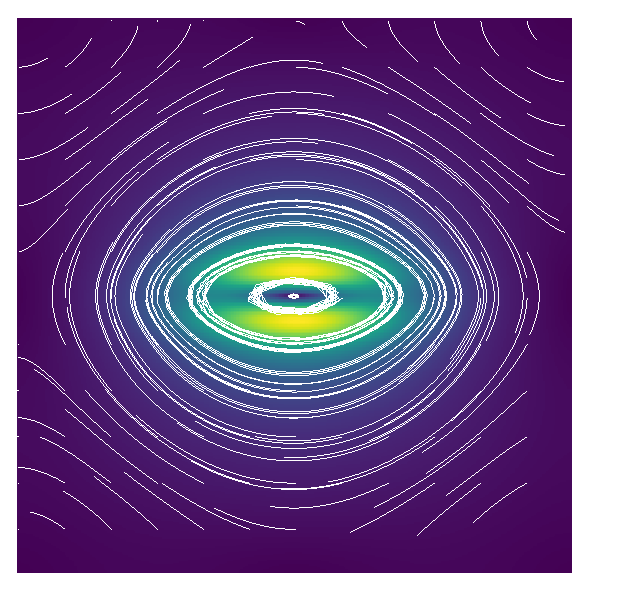
\includegraphics[width=\textwidth, angle=0]{metsim_uniform_rk4.eps}
        \caption{RK4}
    \end{subfigure}
    \caption{Comparison of integration schemes on metsim data. Note the misleading spiral behaviour near the center of the field.}
\end{figure}



\section{Line Integral Convolution}
The LIC algorithm is another method for visualizing vector fields. This method is also based on numerical integration of stream lines,
but does not rely on a seeding strategy. Instead, LIC produces a full visualization at pixel-resolution.

\subsection{Algorithm and implementation}
The same procedure is used to determine the color/intensity of each pixel in the LIC result, which in the simple case is a greyscale image
with resolution equal to the size of the data grid.

The intensity of a pixel $I(u, v)$ is defined as
$$I(u, v) = \int_{-L/2}^{L/2}k(s)N(\sigma_{uv}(s))ds$$
Where $L$ is the kernel length, $k$ is the kernel, $N$ is a noise
texture. $\sigma_{uv}$ is the unique field line passing through the pixel $(u, v)$. Intuitively, each pixel
in the output texture is the result of blurring the noise texture at points along the field line passing through that pixel.
The result is that pixels along the same field line will obtain similar intensities (correlated), while pixels orthogonal to the field line will be uncorrelated.


In the implementation, the computation of the field lines themselves and the convolutions with the kernel happen simultaneously.
The computation is separated into a forward-stepping part and a backward-stepping part.
The implementation (forward part only) in pseudo-code:
\begin{verbatim}
x, y = pixel
for {s = 0; s <= L/2; s++}{
    u_local, v_local = velocity(x, y)
    mag_local = sqrt(u_local**2 + v_local**2) 

    dtx = step_size * u_local / mag_local
    dty = step_size * v_local / mag_local
    x += dtx
    y += dty

    output_texture(x, y) += h[s] * noise_texture(x, y)
}

\end{verbatim}
This is a naive and slow implementation of LIC, though relatively simple to implement.
A major inefficiency is that stream lines are recomputed many times, since many pixels
coincide with the same stream lines.

The algorithm was first implemented in Python (CPU) using numpy to speed up the algorithm. Later, it was reimplemented in Unity, using C\# for pre-processing and HLSL Compute Shaders for the actual LIC implementation.
In the compute shader model, a thread is dispatched for each pixel in the result image, and the shader program executes in parallell across all threads.
This massively sped up execution, and parameters can be changed with almost instant updates. This also made gathering results and fixing bugs much easier.

Simulation and visualization parameters are exposed as shader uniforms and can be changed from the Unity Inspector:
\begin{figure}[h!]
    \centering
    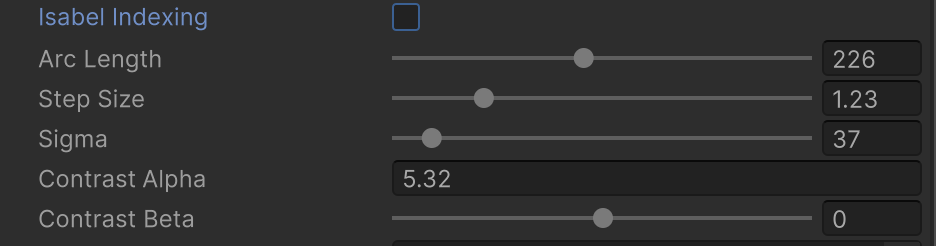
\includegraphics[width=0.75\textwidth]{unity_editor.png}
    \caption{Unity shader uniform interface}
\end{figure}

The datasets are pre-processed and the velocity fields are normalized and encoded into RGB textures.
In the compute shader, the data is sampled and bilinearly filtered on the GPU. The samples must then be "de-normalized"
to obtain the original physically meaningful data values.

Color maps were also added and can be changed by uploading images of the color maps laid out horizontally.
The compute shader simply samples this color-map by using the data-value as a uv-coordinate.

As a post-processing step, the contrast of the LIC image was enhanced by the formula
$$I_{enhanced} = \alpha(I-0.5) + \beta$$

Then, the LIC image was blended with the color-mapped velocity magnitude image using the 
LIC image as an intensity map.

\newpage
\subsection{Results}
First, some basic results are found on both datasets by tuning parameters until the result
was satisfactory.

\begin{figure}[h!]
    \centering
    \begin{subfigure}{0.48\textwidth}
        \centering
        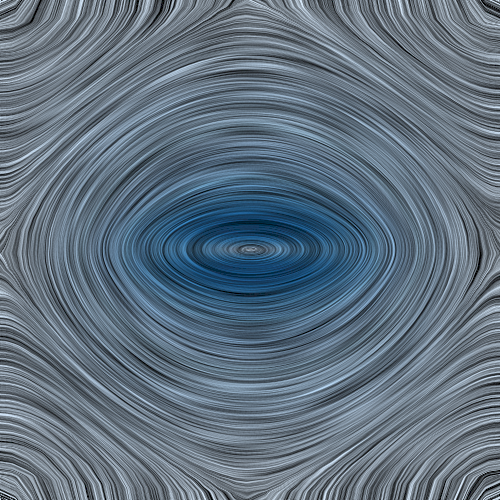
\includegraphics[width=\textwidth]{LIC_metsim.png}
        \caption{Metsim LIC}
    \end{subfigure}
    \hfill
    \begin{subfigure}{0.48\textwidth}
        \centering
        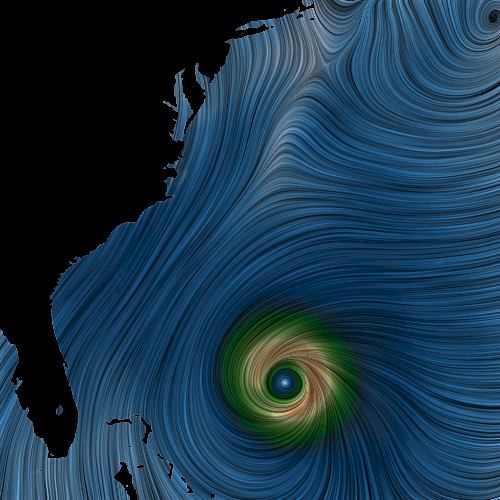
\includegraphics[width=\textwidth]{LIC_isabel.png}
        \caption{Isabel LIC}
    \end{subfigure}
    \caption{}
\end{figure}

\subsubsection{Arc Length}
The algorithm was tested with different arc lengths (constant step length).
\begin{figure}[h!]
    \centering
    \begin{subfigure}{0.30\textwidth}
        \centering
        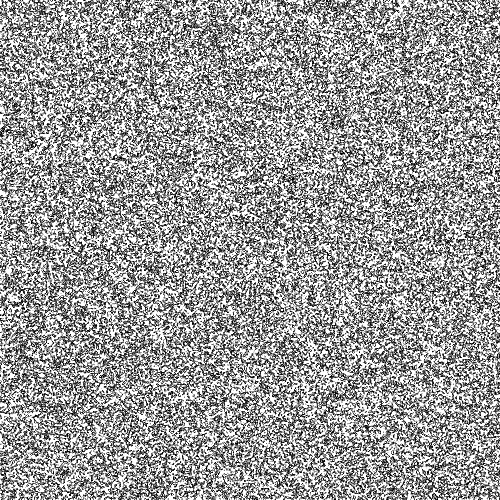
\includegraphics[width=\textwidth]{lic_metsim_arc_1.png}
        \caption{arc length = 1.0}
    \end{subfigure}
    \hfill
    \begin{subfigure}{0.30\textwidth}
        \centering
        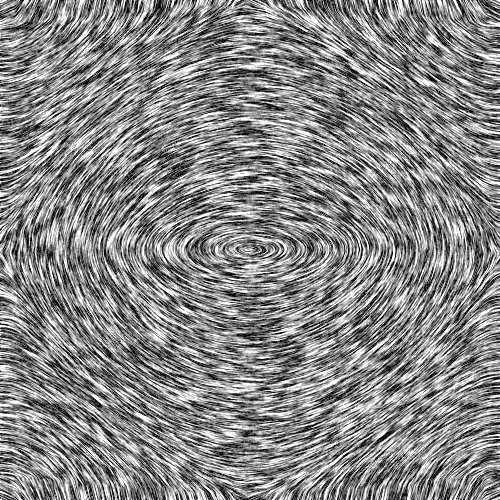
\includegraphics[width=\textwidth]{lic_metsim_arc_8.png}
        \caption{arc length = 8.0}
    \end{subfigure}
    \hfill
    \begin{subfigure}{0.30\textwidth}
        \centering
        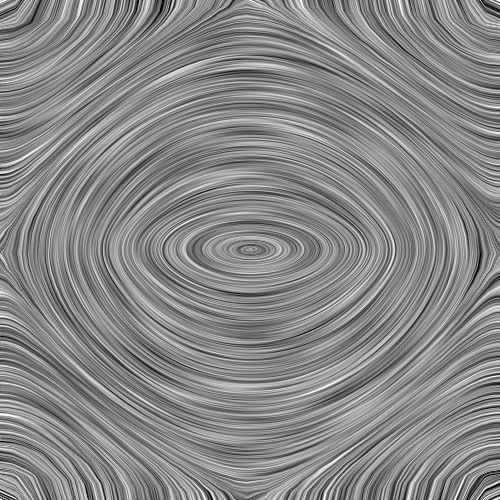
\includegraphics[width=\textwidth]{lic_metsim_arc_50.png}
        \caption{arc length = 50.0}
    \end{subfigure}
    \caption{LIC algorithm on metsim data with different arc lengths.}
\end{figure}

As expected, the LIC image is indistinguishable from the pure noise image when the arc length is too low.
As the arc length increases, the image becomes more and more coherent as the structures grow longer. The performance/efficiency scales approximately 
linearly with the arc length, as this effectively just controls the length of the integration loop. Still, execution is still 
relatively quick (15ms or less with reasonable parameters) when executed using compute shaders.

\begin{figure}[h!]
    \centering
    \begin{subfigure}{0.30\textwidth}
        \centering
        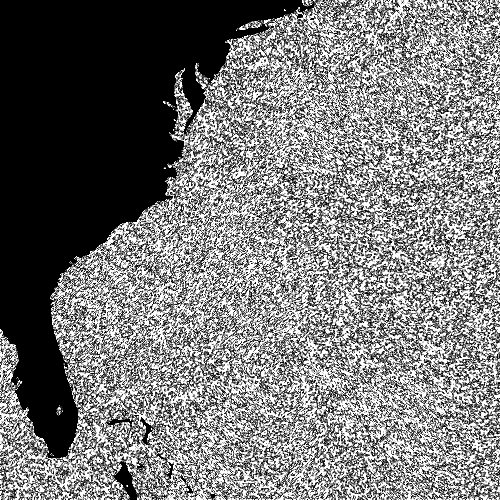
\includegraphics[width=\textwidth]{LIC_isabel_arc_length_1.png}
        \caption{arc length = 1.0}
    \end{subfigure}
    \hfill
    \begin{subfigure}{0.30\textwidth}
        \centering
        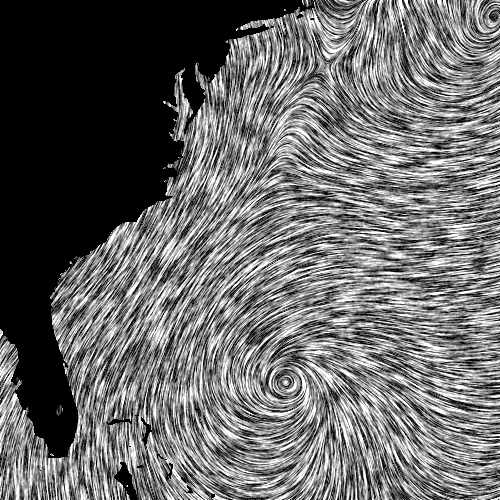
\includegraphics[width=\textwidth]{LIC_isabel_arc_length_8.png}
        \caption{arc length = 8.0}
    \end{subfigure}
    \hfill
    \begin{subfigure}{0.30\textwidth}
        \centering
        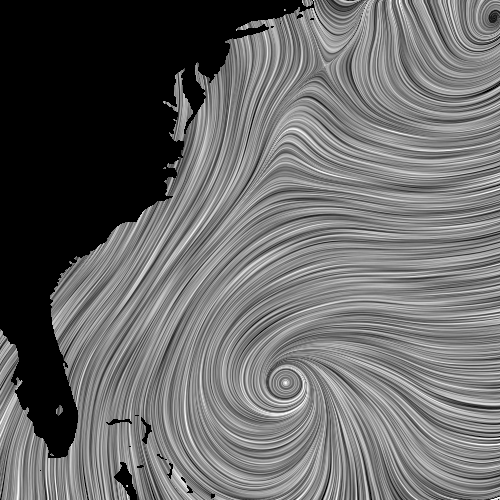
\includegraphics[width=\textwidth]{LIC_isabel_arc_length_50.png}
        \caption{arc length = 50.0}
    \end{subfigure}
    \caption{LIC algorithm on isabel data with different arc lengths.}
\end{figure}

\subsubsection{Euler vs. RK4 on LIC}
To test LIC's robustness to simulation errors, results using the RK4 and Euler methods were gathered.
 
\begin{figure}[h!]
    \centering
    \begin{subfigure}{0.48\textwidth}
        \centering
        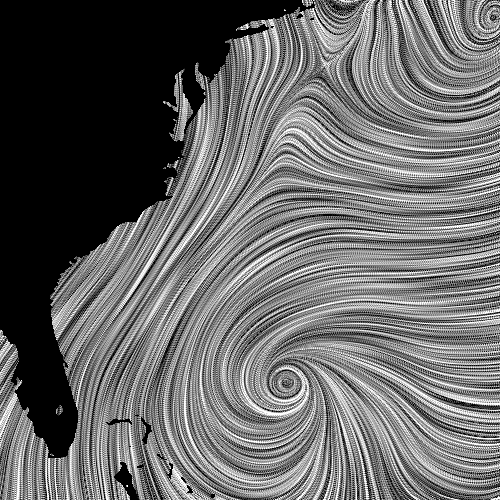
\includegraphics[width=\textwidth]{isabel_euler.png}
        \caption{Euler scheme}
    \end{subfigure}
    \hfill
    \begin{subfigure}{0.48\textwidth}
        \centering
        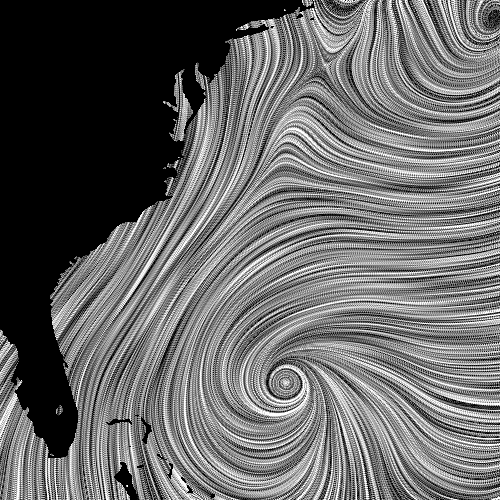
\includegraphics[width=\textwidth]{isabel_rk4.png}
        \caption{RK4 scheme}
    \end{subfigure}
\end{figure}

\begin{figure}[h!]
    \centering
    \begin{subfigure}{0.48\textwidth}
        \centering
        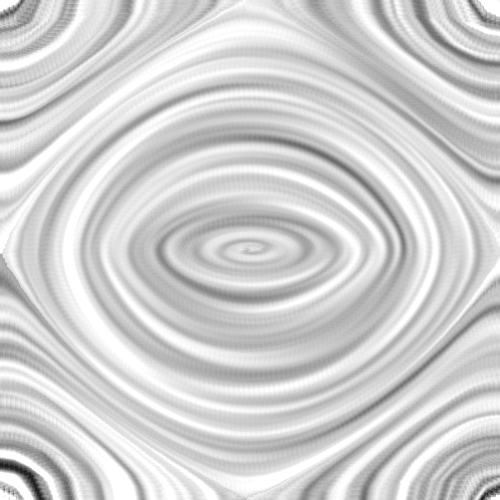
\includegraphics[width=\textwidth]{lic_metsim_euler.png}
        \caption{Euler scheme}
    \end{subfigure}
    \hfill
    \begin{subfigure}{0.48\textwidth}
        \centering
        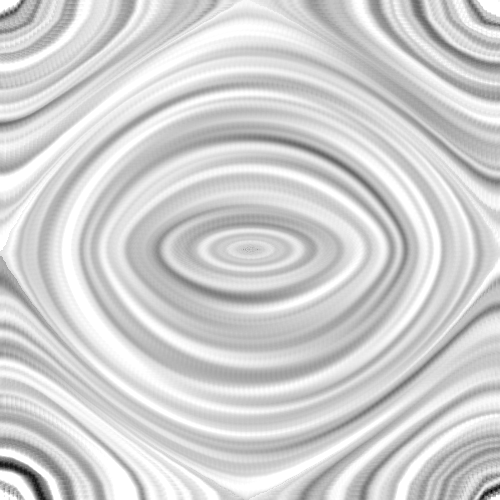
\includegraphics[width=\textwidth]{lic_metsim_rk4.png}
        \caption{RK4 scheme}
    \end{subfigure}
\end{figure}

While not immediately obvious from these images, the RK4 scheme produces finer details in the structures, particularly in the eye of the hurricane.
In the metsim data, we again see that the euler method results in a spiral-like structure, while the RK4 scheme preserves the elliptical form of the structure.
The step sizes in these images were deliberately kept relatively large to exacerbate the inaccuracy of the Euler scheme.



\newpage 
\subsubsection{Changing resolutions in the metsim dataset}
The metsim dataset has a low intrinsic resolution. This naturally produces a very coarse LIC representation. We can arbitrarily upscale
the vector field (using bilinear interpolation) to produce a smoother result. The figure shows the LIC from the original resolution and from an upscaled version.
The upscaling was done using opencv2.

\begin{figure}[h!]
    \centering
    \begin{subfigure}{0.32\textwidth}
        \centering
        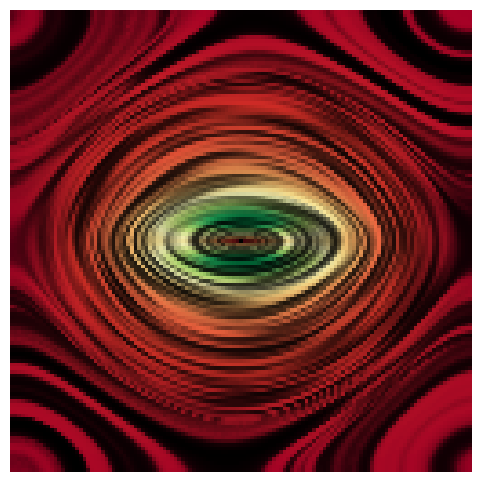
\includegraphics[width=\textwidth]{metsim_original.png}
        \caption{127x126}
    \end{subfigure}
    \hfill
    \begin{subfigure}{0.32\textwidth}
        \centering
        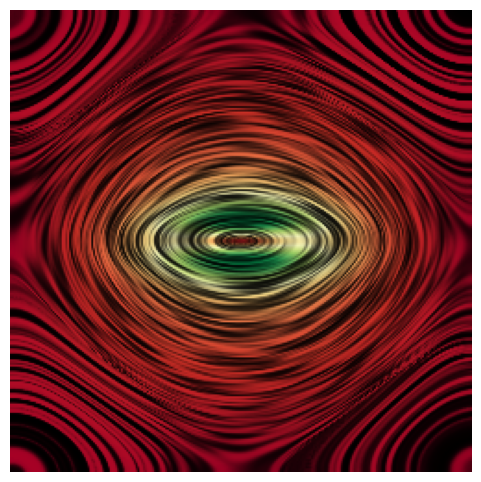
\includegraphics[width=\textwidth]{metsim_250_250.png}
        \caption{250x250}
    \end{subfigure}
    \hfill
    \begin{subfigure}{0.32\textwidth}
        \centering
        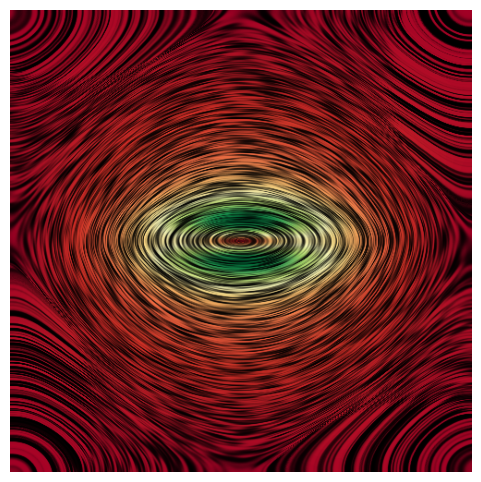
\includegraphics[width=\textwidth]{metsim_500_500.png}
        \caption{500x500}
    \end{subfigure}
    \caption{}
\end{figure}

\section{Geometric vs. Texture-based Methods}
Although this may not be obvious from the results presented, texture-based methods like LIC are inherently more robust to numerical errors than streamline techniques. LIC relies on localized convolution rather than explicit trajectory integration, making it less sensitive to accumulated errors, step size variations, and inaccuracies in regions with high curvature or discontinuities.
In contrast, streamlines are computed through numerical integration, where small errors accumulate over time and directly distort the visualization. LIC blends information across neighboring regions, intuitively "averaging out" local errors. Since LIC is based on texture filtering rather than long, continuous trajectories, it requires only short integration arcs, further reducing the impact of numerical inaccuracies.

Line-based methods are also more intuitive than LIC, though care must be taken in choosing the right seeding strategy. With line-based methods, it's easy to miss
important structures in the data, as large areas of the vector field are totally disregarded. LIC is more complete in this sense, where strong features and critical points
appear naturally through evaluating the entire field/all pixels.

In general, both methods can produce satisfying visualizations of vector fields, and they are
both very flexible. In line-based visualization, a plethora of seeding strategies can be used to produce different results.
In LIC, different input textures, kernel sizes and sub-arc lengths can be experimented with.

Both methods are easily parallellizable, as the same algorithm is used for all elements (seeds for lines, pixels for LIC). 

In a standard, linear CPU implementation, the streamline method was faster to execute, as the number of seeds is only a fraction of the number of pixels. In LIC however, all pixels must be processed, which is slow in a linear implementation.
However, if the algorithm is parallellized, LIC could actually be more performant than streamlines, since the performance bottleneck is in the individual thread execution time, and streamlines typically require a longer integration loop. 
A parallellized streamline algorithm was not implemented, so this was not tested.

\section{Summary and Conclusion}
This report explored methods for visualizing vector fields using field lines and Line Integral Convolution (LIC). Various seeding strategies were tested for field lines: random, uniform, and vorticity-based seeding. Numerical integration methods, Euler and RK4, were compared, with RK4 being more accurate especially regions of high vorticity.

LIC was implemented as a texture-based approach, producing a dense, high-resolution visualization. The effects of kernel length and arc length were examined, demonstrating their influence on image quality. Compared to field lines, LIC provides a more complete visualization but requires higher computational effort.


\section*{Links to code}
\href{https://github.com/edvartGB/visualization/blob/main/oblig/lic_vectorized.ipynb}{Line integral convolution}

\noindent \href{https://github.com/edvartGB/visualization/blob/main/oblig/oblig.ipynb}{Stream lines}

\end{document}
